\section{Einführung in die Finanzwirtschaft}

\textbf{Ziel der Unternehmung}: Unternehmen zielen darauf ab, Wert zu schaffen.

\textbf{Wertschöpfung}: Transformation von Ressourcen in Güter und Dienstleistungen mit höherem Wert. Werte werden meist durch Preise approximiert.

\textbf{Zahlungsströme}:
\begin{center}
	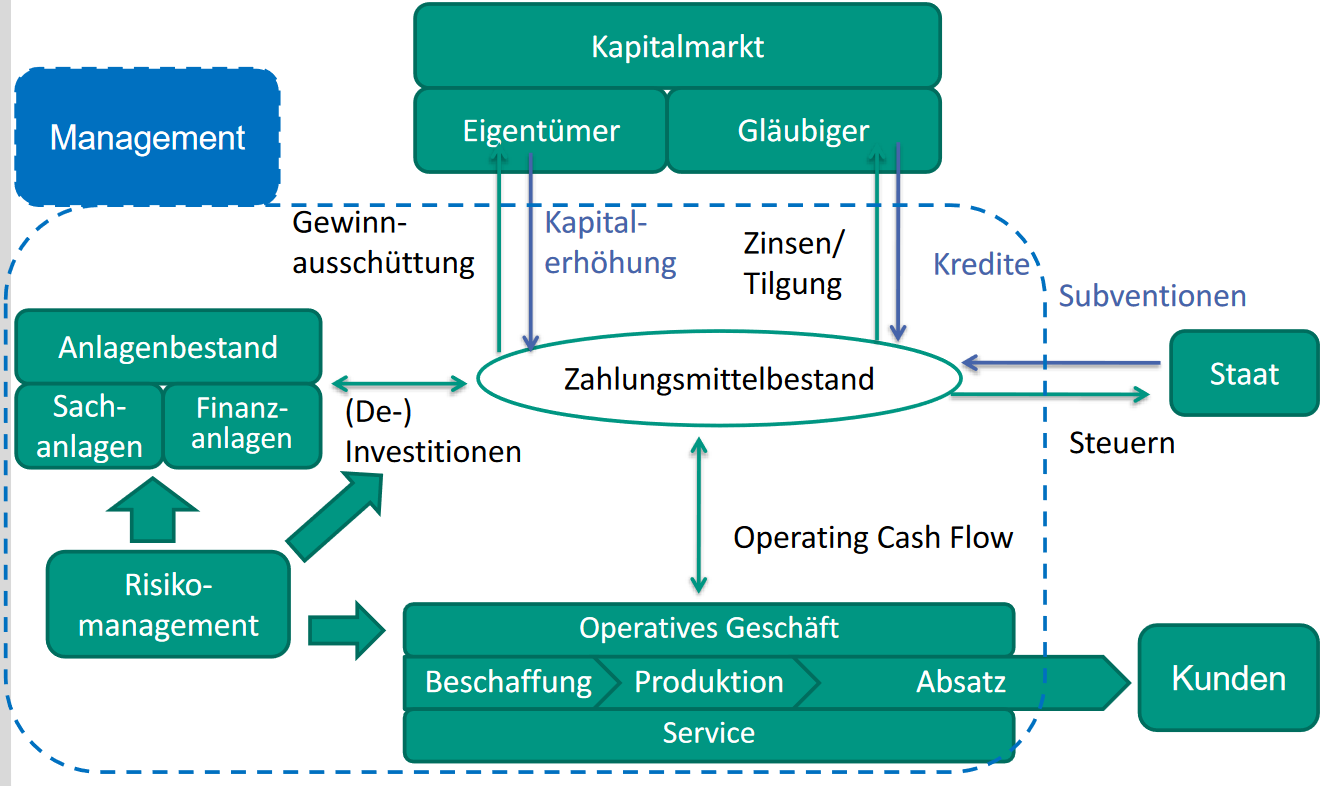
\includegraphics[width=0.8\textwidth]{images/payflow.png}
\end{center}
Aus finanzwirtschaftlicher Sicht ist für eine unternehmerische Entscheidung nur die Frage nach der Wertschöpfung wichtig.
Um unternehmerische Operationen tätigen zu können, wird Kapital benötigt:
\begin{itemize}
	\item Kapitalmarkt führt \textbf{Zahlungen} an das Unternehmen aus
	\item Unternehmen leistet \textbf{Kompensation} für diese Zahlungen
\end{itemize}
\bigskip
\textbf{Zwei finanzwirtschaftliche Entscheidungstypen}:
\begin{itemize}
	\item \textbf{Investition}: Entscheidung, die zunächst eine Auszahlung zur Folge hat
	\begin{itemize}
		\item Implementierung von Projekten, deren Ertrag die Kosten der Finanzierung übersteigt
		\item Kosten der Finanzierung = \textbf{Kapitalkosten}, die auch vom Risiko der Investition abhängen
	\end{itemize}
	\item \textbf{Finanzierung}: Entscheidung, die zunächst einen Kapitalzufluss (Einzahlung) zur Folge hat. Finanzierung üblicherweise durch \textbf{Eigen- und Fremdkapital}.
	\begin{itemize}
		\item \textbf{Eigenkapital}: Nicht-ausgeschüttete Gewinne, Aktien, Ausgabe von Stammanteilen. Kapitalgeber heißt \textbf{Eigentümer}.
		\item \textbf{Fremdkapital}: Kredite, Schuldverschreibungen (Anleihen). Verletzung der vertraglichen Verpflichtungen hat insolvenzrechtliche Konsequenzen. Kapitalgeber heißt \textbf{Gläubiger} und hat bei Insolvenz Vorrang vor den Eigentümern. 
	\end{itemize}
\end{itemize}
\bigskip
\textbf{Wertschöpfung durch geschickte Finanzierung}:
\begin{itemize}
	\item Ausnutzen von institutionellen Verzerrungen, z.B. unterschiedliche Besteuerung der Finanzierungsformen
	\item Vermeidung von riskanten Finanzierungsstrategien
	\item Nutzung von effizienzfördernden Finanzierungsinstrumenten
	\item Ausnutzen von Fehlinformationen oder irrationalem Verhalten von Investoren
\end{itemize}

Jede Entscheidung in einem Unternehmen hat finanzielle Implikationen und fällt in den Bereich der Finanzwirtschaft (\textbf{Corporate Finance}).

Entscheidungen basieren auf einem zweistufigen, quantitativen Vorgehen (\textbf{Bewertung}):
\begin{enumerate}
	\item Ausdrücken aller Konsequenzen einer Entscheidung in Zahlungen
	\item Aggregation aller Zahlungen
\end{enumerate}
$\rightarrow$ Zahlungen als einzig relevante Größe, versuche auch nichtmonetäre Nutzeneinheiten durch Zahlungen zu beschreiben

\textbf{Verortung der Finanzwirtschaft im Unternehmen}:
\begin{center}
	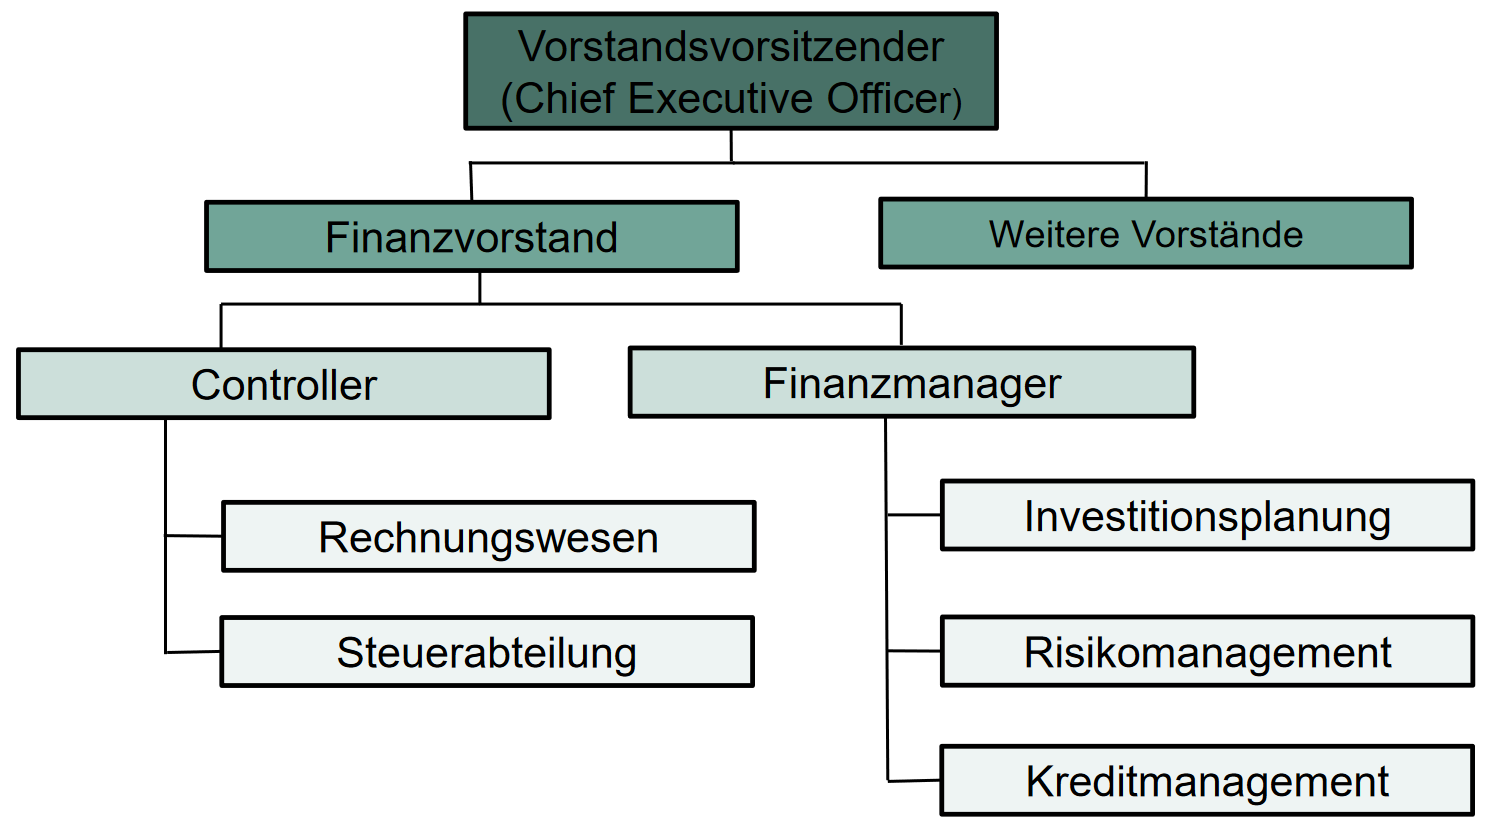
\includegraphics[width=0.8\textwidth]{images/fr-in-comp.png}
\end{center}